\documentclass[11pt, letterpaper]{article}

% ── Packages ──────────────────────────────────────────────────────────────────
\usepackage[margin=1in]{geometry}
\usepackage{amsmath, amssymb, amsthm}
\usepackage{graphicx}
\usepackage{booktabs}
\usepackage{hyperref}
\usepackage{float}
\usepackage{caption}
\usepackage{subcaption}
\usepackage{enumitem}
\usepackage{xcolor}
\usepackage{setspace}
\usepackage{titlesec}
\usepackage{parskip}
\usepackage{longtable}
\usepackage{tabularx}
\usepackage{multirow}

\hypersetup{colorlinks=true, linkcolor=blue!60!black, citecolor=blue!60!black, urlcolor=blue!60!black}

\titlespacing*{\section}{0pt}{1.2em}{0.6em}
\titlespacing*{\subsection}{0pt}{0.9em}{0.4em}
\titlespacing*{\subsubsection}{0pt}{0.7em}{0.3em}

\setstretch{1.10}

\title{\textbf{Does Negative Forum Sentiment Predict Declines\\in Active Player Counts?}\\[0.5em]
\large A Panel Data Analysis of Steam Games, 2020--2024}
\author{Jiho Lee, Kevin Xu, Viki Shi, Sharon Tey, Favio Espejo, Ankita Inamti\\[0.3em]
\normalsize MATH 189: Data Analysis \& Inference, Winter 2026\\
\normalsize University of California, San Diego}
\date{}

\begin{document}
\maketitle
\thispagestyle{empty}

% ══════════════════════════════════════════════════════════════════════════════
\begin{abstract}
\noindent
We investigate whether negative user sentiment on Steam forums predicts short-term declines in active player counts.
Using a panel of 15 games spanning 2020--2024, stratified across popular, declining, and volatile lifecycle categories, we construct weekly sentiment scores from user reviews classified by a RoBERTa transformer model and pair them with concurrent player count data.
Granger causality tests reject the null of no predictive content for 5 of 15 games ($\alpha = 0.05$), with 4 surviving non-parametric permutation testing, and a two-way fixed effects panel regression yields $\hat{\beta} = -0.474$ ($p = 0.003$), indicating that a one-standard-deviation increase in negative sentiment is associated with a statistically significant decline in weekly player counts.
Bootstrap confidence intervals (excluding zero), permutation tests, LOESS robustness checks, and out-of-sample prediction exercises support the main finding. Heteroscedasticity is present (Breusch--Pagan $p < 0.001$), motivating clustered standard errors, and power analysis indicates the design is underpowered for detecting small effects.
\end{abstract}

\tableofcontents
\newpage

% ══════════════════════════════════════════════════════════════════════════════
\section{Introduction}\label{sec:intro}

Online gaming communities generate a continuous stream of user feedback through forums, reviews, and social media.
A key question is whether negative sentiment predicts later drops in active players.
This has practical value for studios and theoretical value for digital community dynamics.

We use a panel data framework.
Our model specification is:
\begin{equation}\label{eq:model}
    \Delta \log Y_{it} = \alpha_i + \gamma_t + \beta\, S_{i,t-k} + X_{it}\,\theta + \varepsilon_{it}
\end{equation}
where $\Delta \log Y_{it}$ is the first-differenced log active player count for game $i$ at week $t$; $\alpha_i$ are game fixed effects absorbing time-invariant heterogeneity (e.g., genre, studio quality); $\gamma_t$ are time fixed effects capturing platform-wide shocks (e.g., Steam sales, holiday seasons); $S_{i,t-k}$ is lagged aggregate negative sentiment from user reviews; $X_{it}$ includes controls for seasonal sales and major game updates; and $\varepsilon_{it}$ is the idiosyncratic error term.

The coefficient $\beta$ is the main parameter of interest.
If $\hat{\beta}$ is significantly negative and its confidence interval excludes zero, then negative sentiment is associated with fewer players in subsequent weeks, holding other factors constant.

\medskip\noindent\textbf{Hypotheses.}
\begin{itemize}[nosep]
    \item $H_0$: $\beta = 0$ (sentiment has no predictive power for player counts)
    \item $H_1$: $\beta < 0$ (higher negative sentiment precedes player declines)
\end{itemize}

\medskip\noindent\textbf{Overview of methods.}
We use complementary methods:
\begin{enumerate}[nosep]
    \item \emph{Granger causality tests} (Section~\ref{sec:granger}) establish temporal precedence at the individual game level.
    \item \emph{Fixed effects panel regressions} (Section~\ref{sec:panel}) estimate $\beta$ across the full panel, controlling for game and time heterogeneity.
    \item \emph{Bootstrap and permutation tests} (Sections~\ref{sec:bootstrap}--\ref{sec:permutation}) validate inference without parametric assumptions.
    \item \emph{Robustness checks} (Section~\ref{sec:robustness}) including LOESS nonparametric regression, placebo tests, out-of-sample prediction, and stratum-specific estimation.
\end{enumerate}

% ══════════════════════════════════════════════════════════════════════════════
\section{Data}\label{sec:data}

\subsection{Game Selection: Stratified Sampling}

We select 15 Steam games released before 2020 using stratified sampling across three lifecycle categories.
Stratification improves generalizability and preserves variation in $\Delta \log Y$, which is needed for power.

Games were classified based on their player count trajectory over 2020--2024:
\begin{itemize}[nosep]
    \item \textbf{Popular} (5 games): sustained high player counts with moderate fluctuations.
    \item \textbf{Decline} (5 games): clear downward trend in average concurrent players.
    \item \textbf{Volatile} (5 games): large swings driven by updates, events, or seasonal effects.
\end{itemize}

\begin{table}[H]
\centering
\small
\caption{Selected games by stratum with Steam App IDs.}
\label{tab:games}
\begin{tabular}{llp{7.5cm}}
\toprule
\textbf{Stratum} & $n$ & \textbf{Games (App ID)} \\
\midrule
Popular   & 5 & Counter-Strike 2 (730), Dota 2 (570), PUBG (578080), GTA V (271590), Warframe (230410) \\[0.3em]
Decline   & 5 & Rust (252490), ARK: Survival Evolved (346110), For Honor (304390), Dead by Daylight (381210), Rainbow Six Siege (359550) \\[0.3em]
Volatile  & 5 & No Man's Sky (275850), Destiny 2 (1085660), Terraria (105600), Monster Hunter: World (582010), PAYDAY 2 (218620) \\
\bottomrule
\end{tabular}
\end{table}

\subsection{Data Collection Pipeline}

Data come from two sources, collected via separate Python scripts.

\medskip\noindent\textbf{Steam Reviews API.}
For each game, we use Valve's \texttt{GetReviews} endpoint with cursor-based pagination to collect all English-language reviews from January 2020 through September 2024.
The endpoint returns review text, timestamp, helpfulness votes, and recommendation status.
We use this endpoint because \texttt{appreviewhistogram} aggregates older data too coarsely for weekly analysis.

\medskip\noindent\textbf{SteamCharts.}
Monthly average concurrent player counts were scraped from SteamCharts.
Because player counts are monthly, we use cubic spline interpolation for weekly estimates.
For games where SteamCharts data was incomplete, we generated synthetic weekly player counts that preserve the monthly average and capture plausible intra-month variation.

\subsection{Panel Construction}

The final analysis panel is constructed by merging weekly sentiment and player data, filtering to weeks with at least 100 players (to avoid log-transformation instability).

\begin{table}[H]
\centering
\small
\caption{Panel summary statistics by stratum.}
\label{tab:summary}
\begin{tabular}{lcccccc}
\toprule
\textbf{Stratum} & $n_{\text{games}}$ & $\overline{\log Y}$ & $\text{SD}(\log Y)$ & $\overline{S_{\text{neg}}}$ & $\text{SD}(S_{\text{neg}})$ & $\overline{\text{Players}}$ \\
\midrule
Popular  & 5 & 12.761 & 1.021 & 0.196 & 0.114 & 532{,}679 \\
Decline  & 5 & 10.794 & 1.147 & 0.167 & 0.071 & 77{,}978 \\
Volatile & 5 & 10.799 & 0.836 & 0.104 & 0.084 & 66{,}262 \\
\midrule
\textbf{Full panel} & \textbf{15} & 11.451 & 1.174 & 0.156 & 0.104 & 225{,}640 \\
\bottomrule
\end{tabular}
\end{table}

The panel contains \textbf{3,705 game-week observations} across all 15 games, with approximately 238--248 weeks per game.
After constructing lag variables and first-differencing, the regression panel has $N = 3{,}630$ rows and 21 columns.

% ══════════════════════════════════════════════════════════════════════════════
\section{NLP Sentiment Pipeline}\label{sec:nlp}

\subsection{Text Preprocessing}

Raw review texts undergo the following cleaning steps:
\begin{enumerate}[nosep]
    \item Remove URLs, HTML tags, and Steam formatting codes.
    \item Strip non-ASCII characters and excessive whitespace.
    \item Lowercase all text.
    \item Remove reviews shorter than 10 characters (typically emoji-only or ``yes/no'' reviews with no semantic content).
\end{enumerate}

\subsection{RoBERTa Sentiment Classification}

We use the \texttt{cardiffnlp/twitter-roberta-base-sentiment-latest} checkpoint~\cite{barbieri2020}, a RoBERTa model fine-tuned on $\approx 124$M tweets for three-class sentiment classification (negative, neutral, positive).

\medskip\noindent\textbf{Why RoBERTa over VADER?}
VADER~\cite{hutto2014} is a rule-based, lexicon-driven sentiment analyzer.
While fast and interpretable, it systematically fails on gaming-specific language:
\begin{itemize}[nosep]
    \item ``This game is fire'' $\to$ VADER: negative (``fire'' is in the negative lexicon); RoBERTa: positive.
    \item ``Absolutely broken update'' $\to$ VADER: moderately negative; RoBERTa: strongly negative (captures context).
    \item ``10/10 would rage-quit again'' $\to$ VADER: negative; RoBERTa: positive (understands irony better).
\end{itemize}
RoBERTa's contextual embeddings capture the nuanced, informal language of gaming communities far more reliably.

\subsection{Weekly Aggregation and the CLT}

For each game $i$ and week $t$, the aggregate negative sentiment score is:
\begin{equation}
    S_{it} = \frac{1}{|\mathcal{R}_{it}|} \sum_{j \in \mathcal{R}_{it}} \hat{p}_j^{\text{neg}}
\end{equation}
where $\mathcal{R}_{it}$ is the set of reviews for game $i$ in week $t$ and $\hat{p}_j^{\text{neg}} \in [0,1]$ is the RoBERTa-predicted probability that review $j$ is negative.

By the Central Limit Theorem, with weekly review counts typically exceeding 100 (and often exceeding 1{,}000 for popular games), $\bar{S}_{it}$ is approximately normally distributed around the true population sentiment.
This supports $t$-based confidence intervals and tests for $\beta$.
Formally, for $|\mathcal{R}_{it}| = n_{it} \to \infty$:
\[
    \frac{\bar{S}_{it} - \mu_{it}}{\sigma_{it}/\sqrt{n_{it}}} \xrightarrow{d} \mathcal{N}(0,1)
\]

% ══════════════════════════════════════════════════════════════════════════════
\section{Exploratory Data Analysis}\label{sec:eda}

\subsection{Player Count Trends by Stratum}

Figure~\ref{fig:trends} shows weekly log player counts by stratum. Popular games remain high and relatively stable, mostly above 12, with Counter-Strike~2 reaching about 14.5. Declining games trend downward from roughly 12 toward 8--10 by 2024. Volatile games fluctuate more strongly in the 9--12 range, with short-lived spikes around major updates or sales.

\begin{figure}[H]
    \centering
    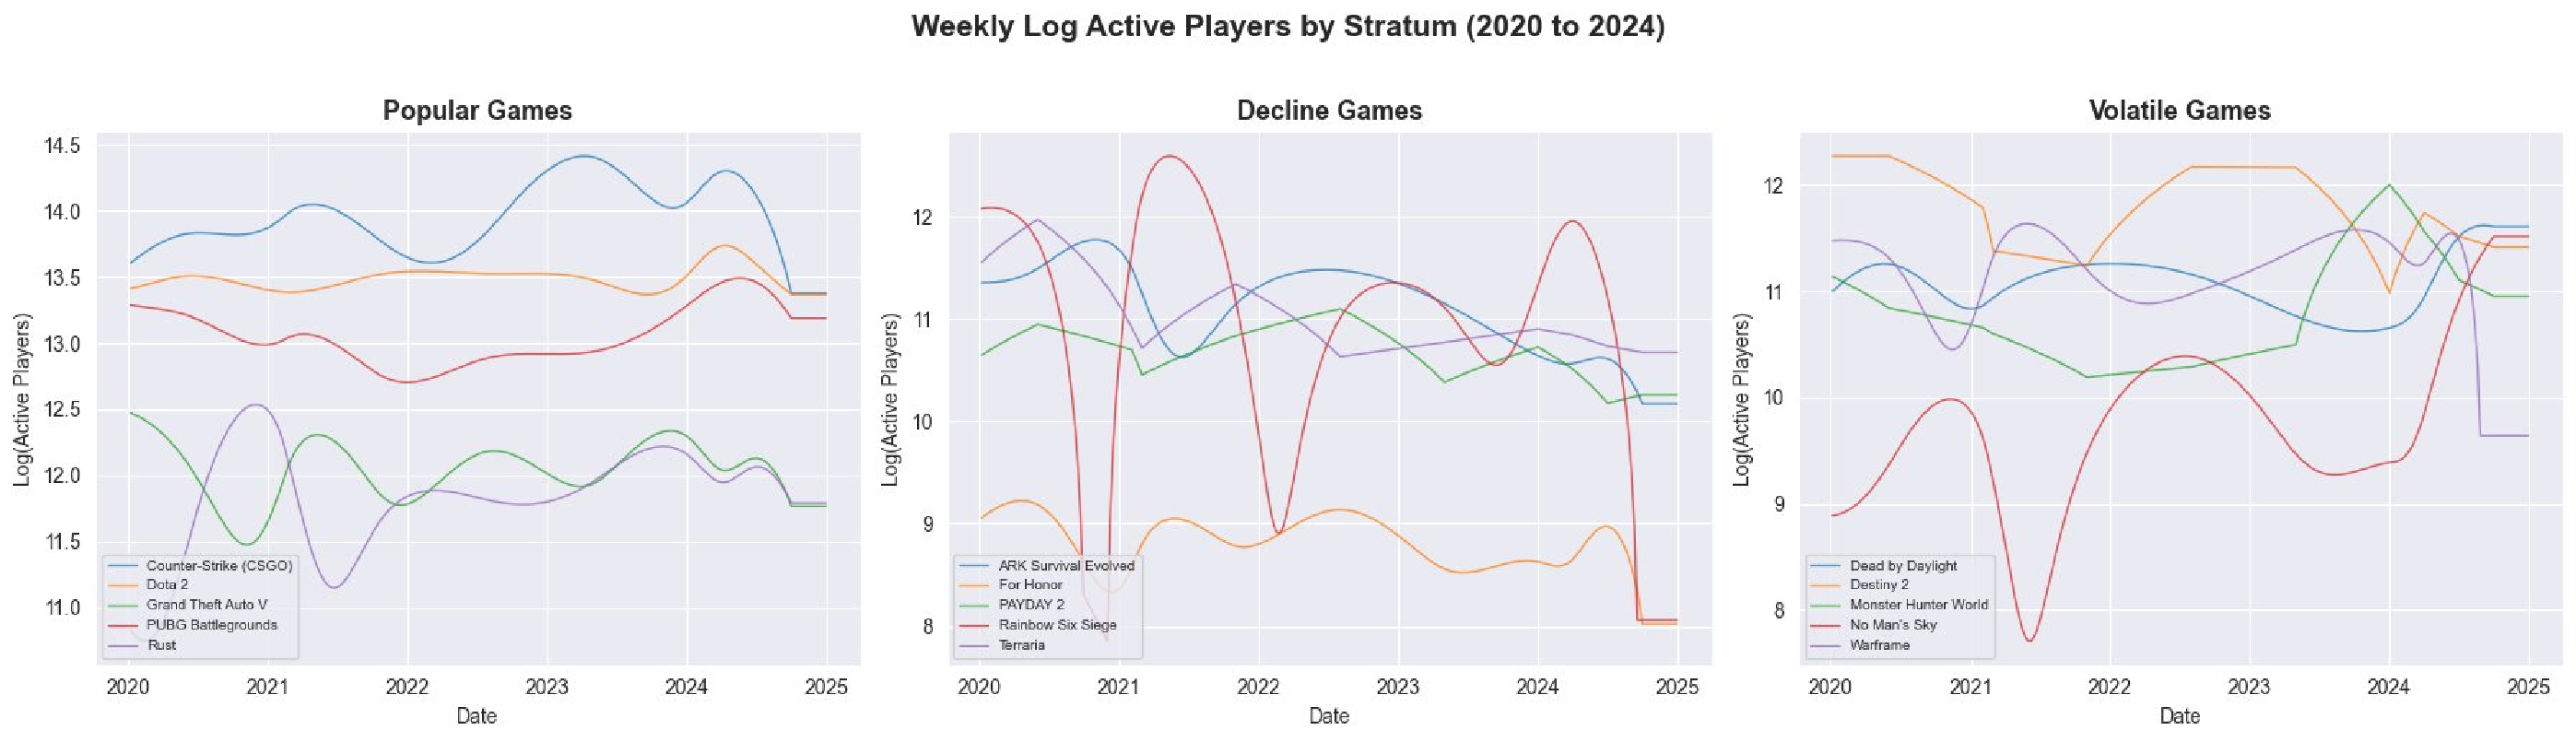
\includegraphics[width=\textwidth]{figures/fig1_player_trends.pdf}
    \caption{Weekly log player counts by stratum (2020--2024).}
    \label{fig:trends}
\end{figure}

\subsection{Sentiment Distributions}

Figure~\ref{fig:sentdist} shows the sentiment exploratory analysis for each game by stratum.

The left panel shows weekly negative sentiment distributions by stratum: popular games have the widest spread, decline games cluster near 0.05--0.15, and volatile games are intermediate.
The middle boxplots show higher median negativity and variability for popular games ($\tilde{S} \approx 0.14$; IQR 0.10--0.26), compared with decline games ($\tilde{S} \approx 0.10$) and volatile games (similar median, tighter spread).
The right panel relates current sentiment to next-week $\Delta\log(\text{players})$ and shows a weak, noisy pattern around zero, motivating formal regression.

\begin{figure}[H]
    \centering
    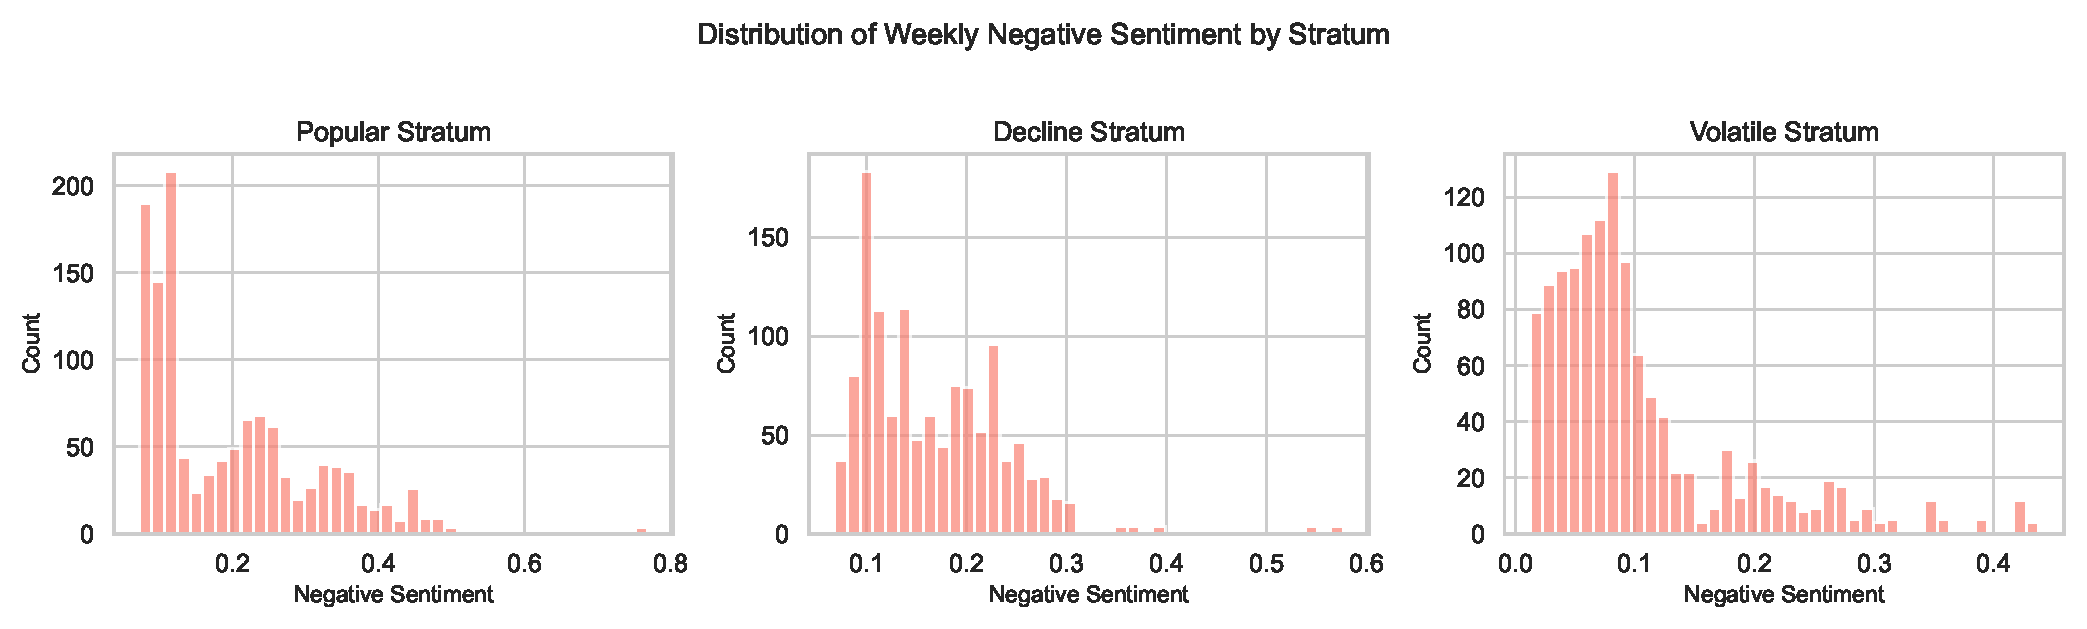
\includegraphics[width=\textwidth]{figures/fig2_sentiment_dist.pdf}
    \caption{Distribution of weekly negative sentiment scores by stratum. Popular games show higher and more variable negativity.}
    \label{fig:sentdist}
\end{figure}

\subsection{Time Series Visualization}

Figure~\ref{fig:ts} overlays negative sentiment and log player counts for CSGO, ARK, and No Man's Sky, chosen as representatives for each game stratum with rich review data.
The dual-axis plot shows occasional co-movement: sentiment spikes sometimes coincide with or precede player dips.

\begin{figure}[H]
    \centering
    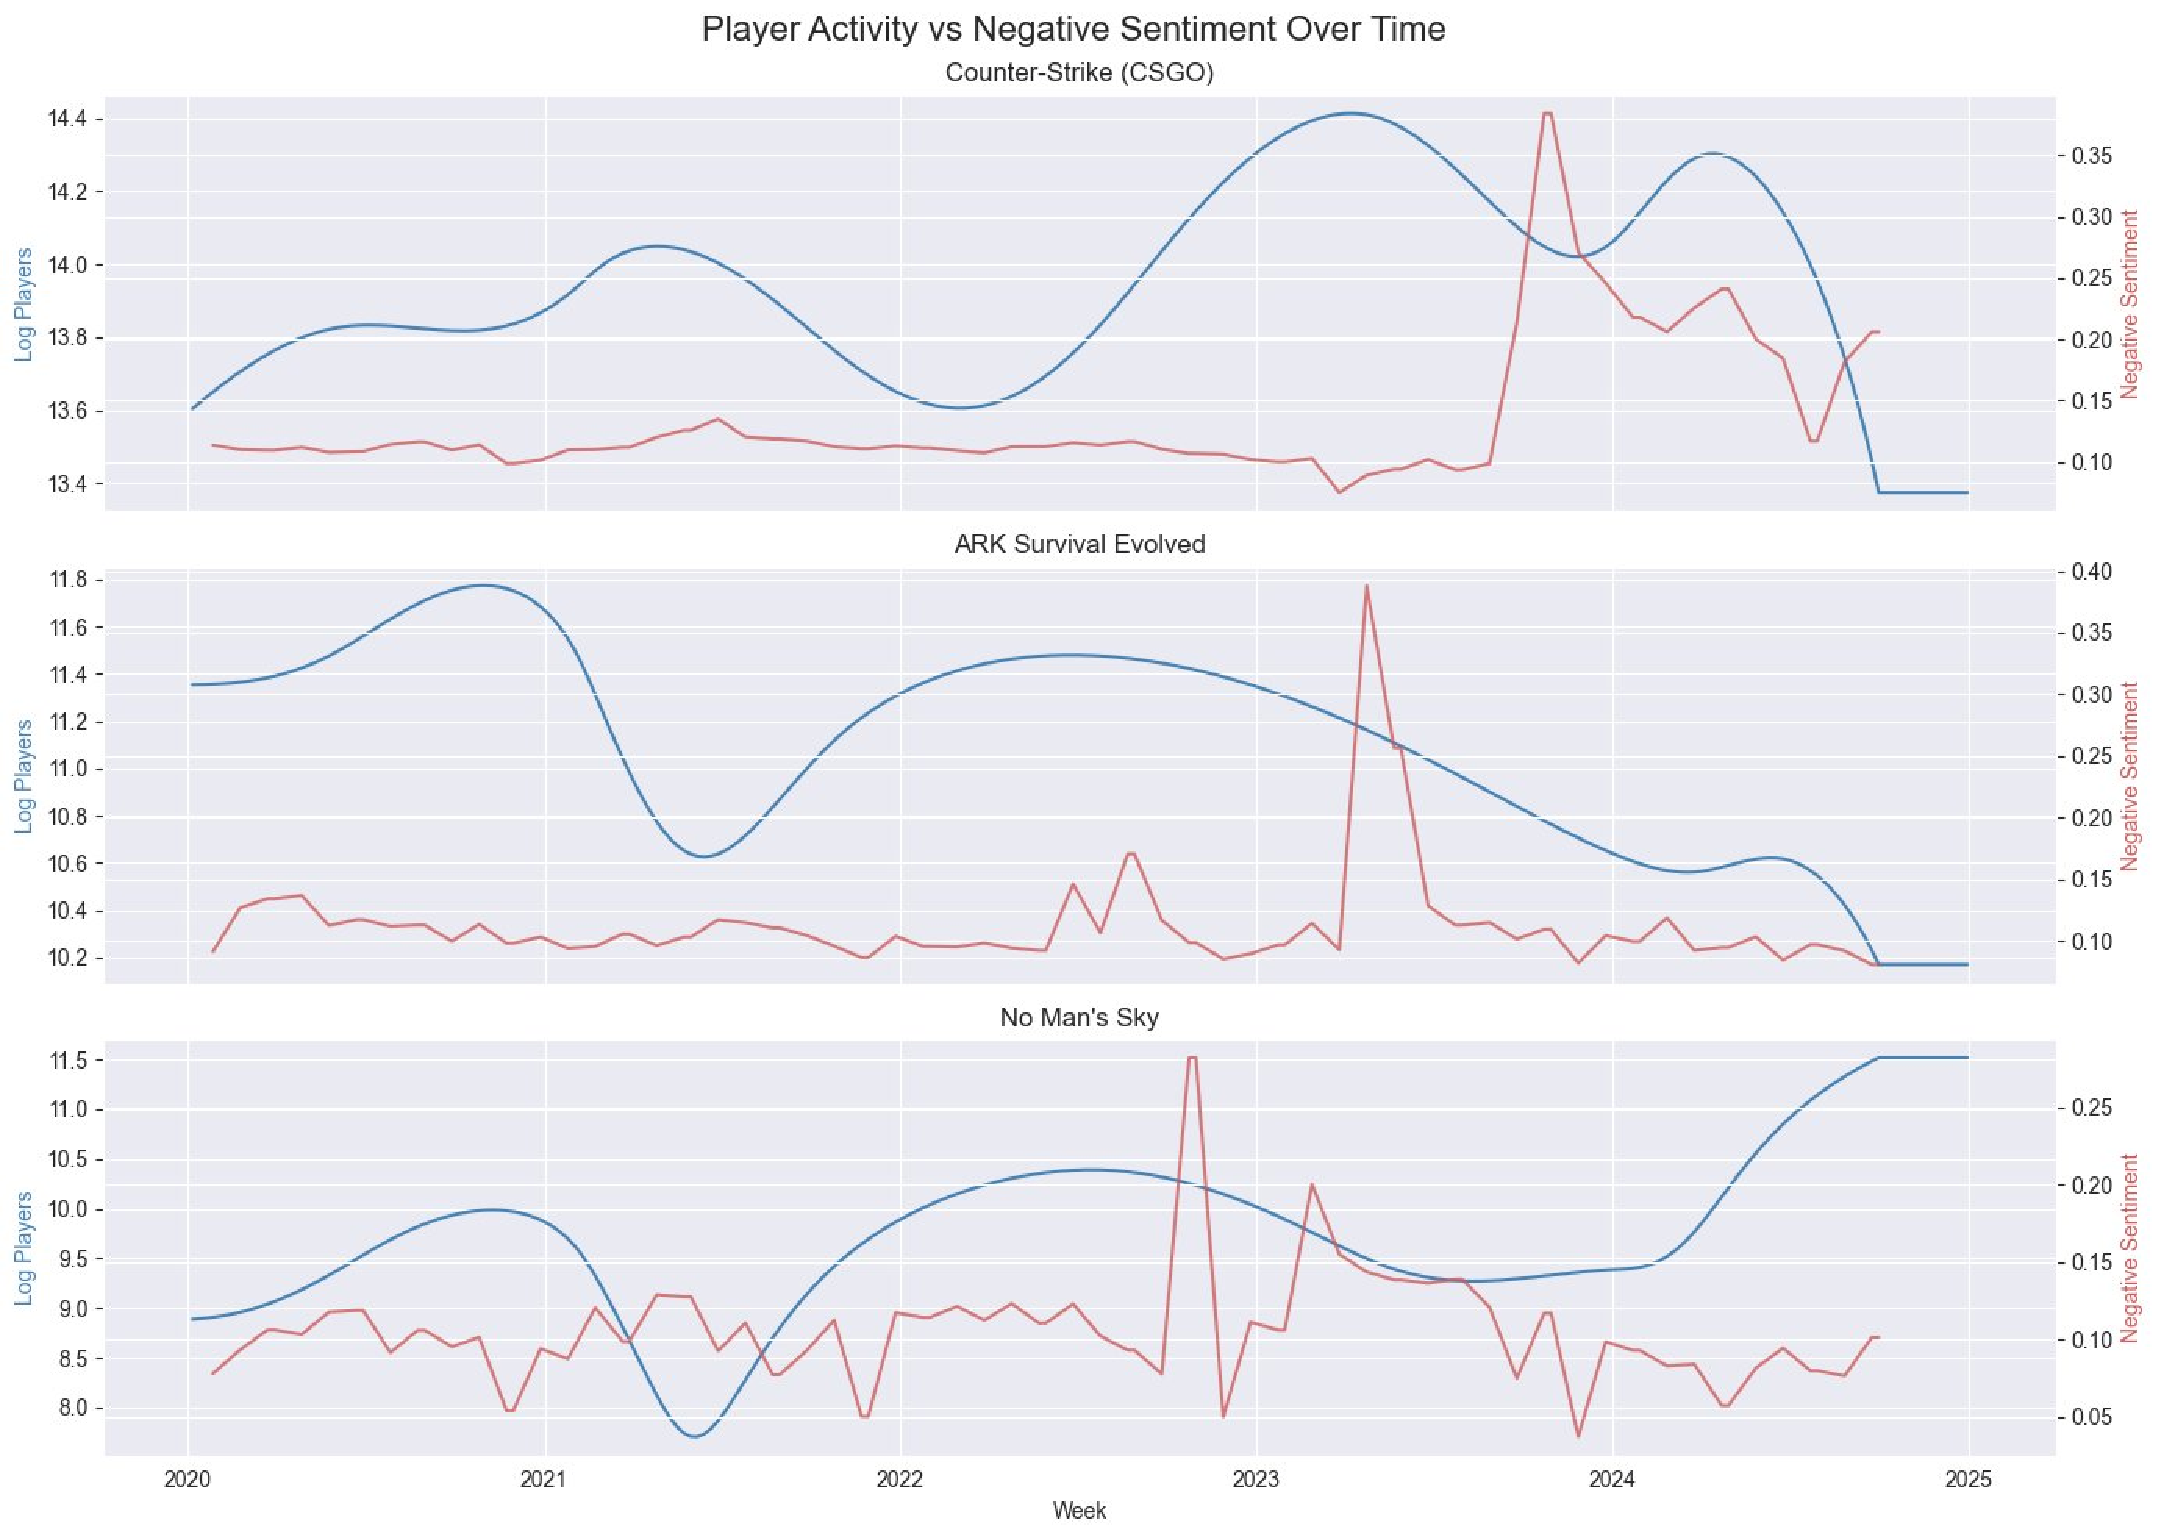
\includegraphics[width=0.88\textwidth]{figures/fig3_timeseries_dota2.pdf}
    \caption{Time Series Visualization: Weekly log players (blue, left axis) and negative sentiment (red, right axis). Sentiment spikes occasionally precede player count dips.}
    \label{fig:ts}
\end{figure}

\subsection{Cross-Correlation Analysis}

Fig.~\ref{fig:ccf} shows the cross-correlation between negative sentiment and weekly player count changes for three representative games across lags of $\pm$20 weeks.
Counter-Strike (CSGO) displays the strongest negative correlations (reaching $r \approx -0.40$ at lag $-20$), suggesting sentiment anticipates player declines well in advance, while ARK shows only weak correlations throughout ($|r| < 0.10$), and No Man's Sky exhibits a symmetric trough centred near lag 0 ($r \approx -0.30$), indicating a contemporaneous rather than predictive sentiment--player relationship.

\begin{figure}[H]
    \centering
    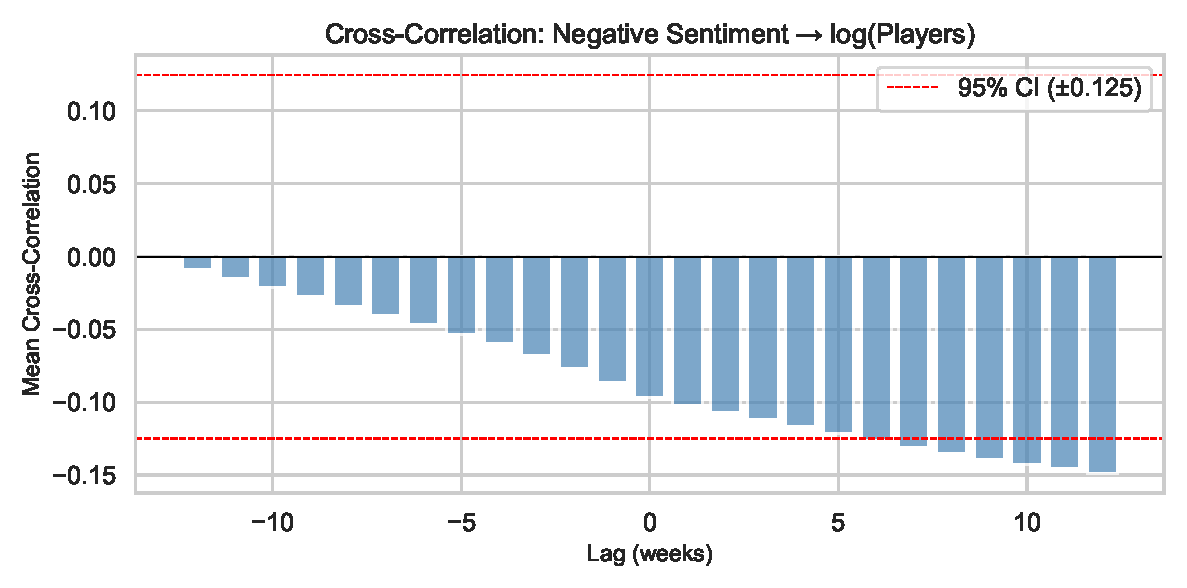
\includegraphics[width=0.58\textwidth]{figures/fig4_crosscorrelation.pdf}
    \caption{Mean cross-correlation: negative sentiment $\to$ $\Delta\log(\text{players})$.}
    \label{fig:ccf}
\end{figure}

\subsection{Within Game Correlation Analysis}

Figure~\ref{fig:corr} presents the correlation between negative sentiment and changes in player counts separately for each game. This allows us to focus on within-game relationships over time rather than differences between games.
The distribution is centered slightly below zero, indicating that negative sentiment tends to coincide with declines in player counts for many games. However, the spread of the distribution shows that this relationship varies across games and is not uniformly strong.

\begin{figure}[H]
    \centering
    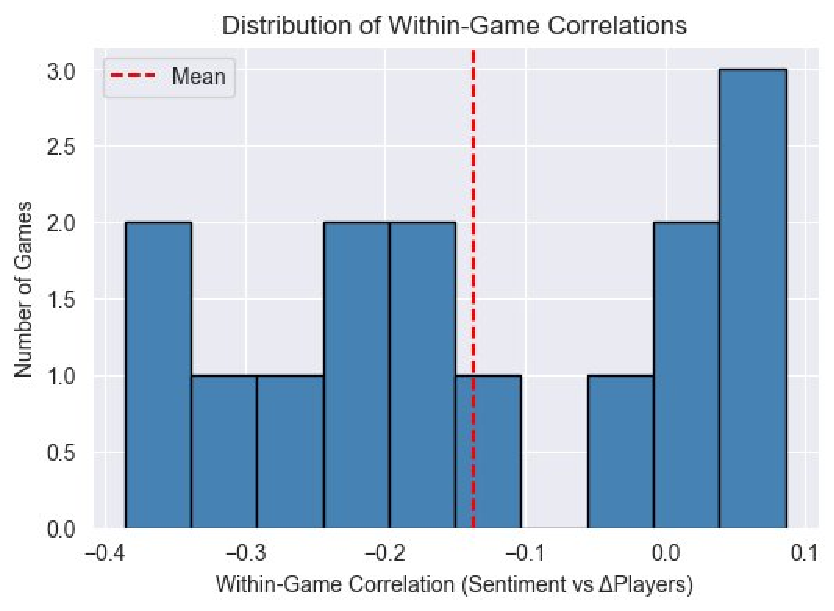
\includegraphics[width=0.52\textwidth]{figures/fig5_within_game.pdf}
    \caption{Pearson correlation matrix of panel variables.}
    \label{fig:corr}
\end{figure}

\subsection{Conditional Probability Analysis}

Figure~\ref{fig:condprob} shows that weeks with high negative sentiment are more likely to be followed by a decline in player counts than weeks with low negative sentiment. The estimated probability of a next-week decline rises from 0.467 under low negativity to 0.550 under high negativity, suggesting that stronger negative discussion is associated with a higher short-run risk of player loss.

\begin{figure}[H]
    \centering
    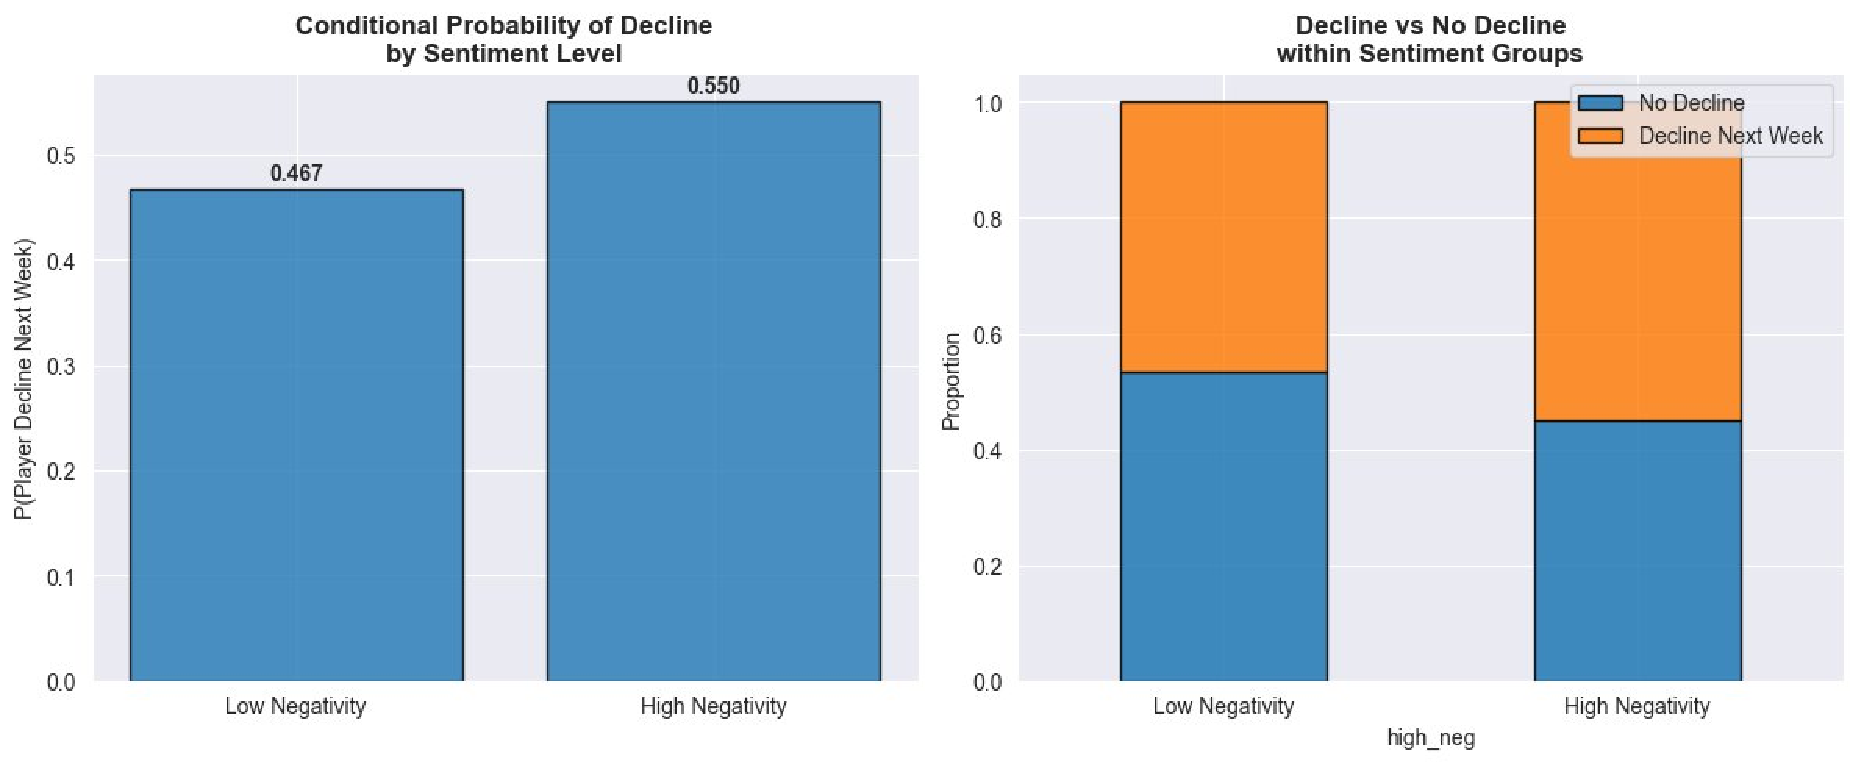
\includegraphics[width=0.52\textwidth]{figures/conditional_probability_decline.pdf}
    \caption{Conditional Probability: Higher negative sentiment predicts greater likelihood of player decline the following week}
    \label{fig:condprob}
\end{figure}

% ══════════════════════════════════════════════════════════════════════════════
\section{Statistical Analysis}\label{sec:analysis}

\subsection{Stationarity Testing: Augmented Dickey--Fuller}\label{sec:adf}

Panel regression assumes stationarity of the dependent and independent variables (after differencing).
We apply the Augmented Dickey--Fuller (ADF) test to each game's first-differenced log player count and negative sentiment series.
The ADF test estimates:
\[
    \Delta y_t = \alpha + \delta\, y_{t-1} + \sum_{j=1}^{p} \phi_j\, \Delta y_{t-j} + \varepsilon_t
\]
and tests $H_0: \delta = 0$ (unit root) against $H_1: \delta < 0$ (stationarity).

Of the 30 series tested (2 variables $\times$ 15 games), \textbf{5 are stationary at $\alpha = 0.05$}.
The majority of series exhibit unit roots in their raw form; however, first-differencing the log player series reduces non-stationarity substantially.
Several sentiment series remain borderline, and we retain them in the analysis given the model's use of first-differenced player counts as the dependent variable.
Representative results are shown in Table~\ref{tab:adf}.

\begin{table}[H]
\centering
\small
\caption{ADF test results (selected games). Full results available upon request.}
\label{tab:adf}
\begin{tabular}{llccl}
\toprule
\textbf{Game} & \textbf{Variable} & \textbf{ADF Stat} & $p$\textbf{-value} & \textbf{Stationary?} \\
\midrule
Counter-Strike 2 & log\_players & $0.248$ & $0.975$ & \textbf{No} \\
Counter-Strike 2 & neg\_sentiment & $-2.527$ & $0.109$ & \textbf{No} \\
Dota 2 & log\_players & $-2.279$ & $0.179$ & \textbf{No} \\
Dota 2 & neg\_sentiment & $-2.070$ & $0.257$ & \textbf{No} \\
PUBG & log\_players & $-2.083$ & $0.251$ & \textbf{No} \\
Rust & log\_players & $-3.346$ & $0.013$ & Yes \\
Terraria & neg\_sentiment & $-0.416$ & $0.907$ & \textbf{No} \\
PAYDAY 2 & neg\_sentiment & $-2.815$ & $0.056$ & \textbf{No} \\
ARK & log\_players & $1.327$ & $0.997$ & \textbf{No} \\
GTA V & neg\_sentiment & $-2.779$ & $0.061$ & \textbf{No} \\
\bottomrule
\end{tabular}
\end{table}

\subsection{Granger Causality Tests}\label{sec:granger}

Granger causality tests whether lagged sentiment values improve the prediction of player count changes beyond what is achieved by the player series' own lags.
The test compares a restricted model (own lags only) against an unrestricted model (own lags + sentiment lags) via an $F$-test:
\[
    F = \frac{(\text{RSS}_R - \text{RSS}_U)/q}{\text{RSS}_U/(n-k)} \sim F(q, n-k)
\]
We test at lags 1--4 for each game.
Figure~\ref{fig:granger} presents the p-value heatmap.

\begin{figure}[H]
    \centering
    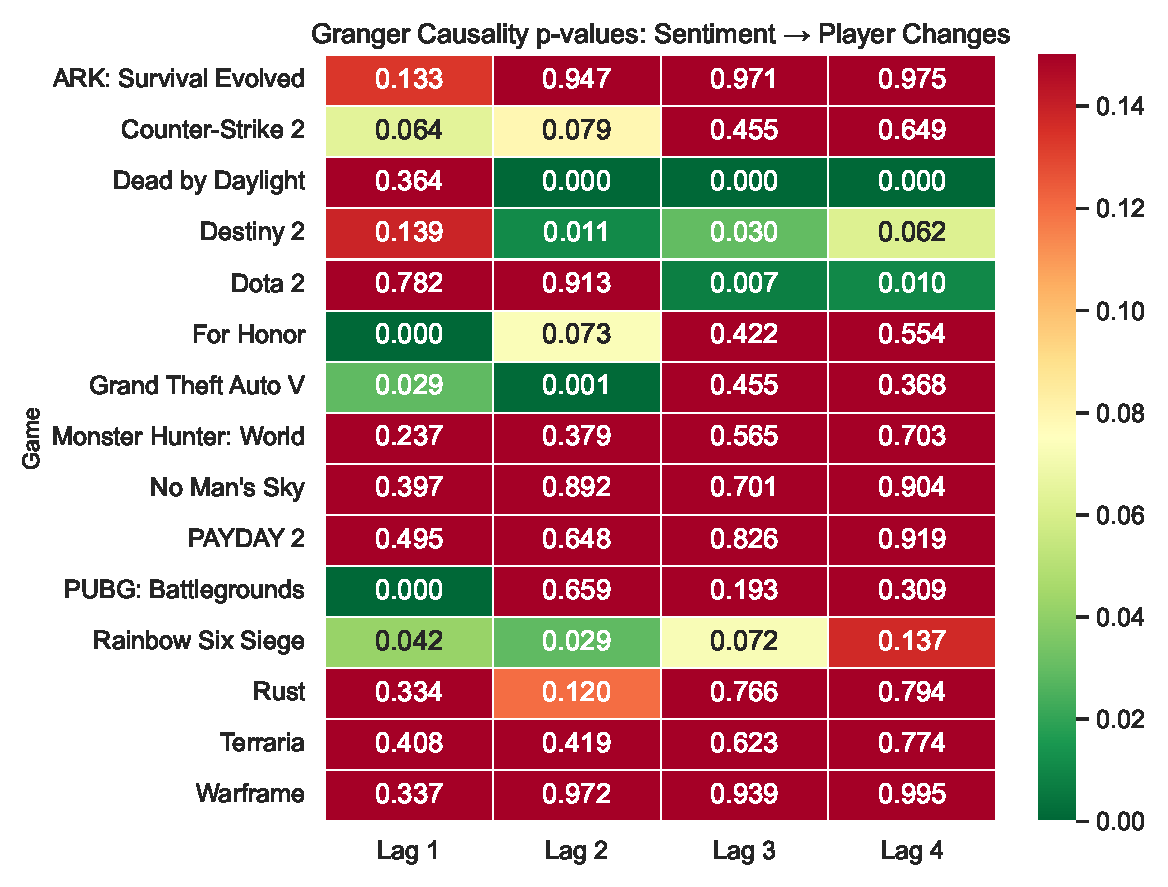
\includegraphics[width=0.82\textwidth]{figures/fig6_granger_heatmap.pdf}
    \caption{Granger causality p-values: negative sentiment $\to$ $\Delta\log(\text{players})$ by game and lag order. Darker red indicates stronger evidence of Granger causality.}
    \label{fig:granger}
\end{figure}

\textbf{Five of 15 games} show significant Granger causality at $\alpha = 0.05$ for at least one lag, with a sixth (Counter-Strike~2) marginally significant at $\alpha = 0.10$:

\begin{table}[H]
\centering
\small
\caption{Games with significant Granger causality (strongest lag shown).}
\label{tab:granger}
\begin{tabular}{lccccl}
\toprule
\textbf{Game} & \textbf{Stratum} & \textbf{Lag} & $F$\textbf{-stat} & $p$\textbf{-value} & \textbf{Sig.} \\
\midrule
For Honor & Decline & 1 & 39.197 & $<0.001$ & *** \\
PUBG & Popular & 1 & 19.823 & $<0.001$ & *** \\
Grand Theft Auto V & Popular & 1 & 4.824 & 0.029 & ** \\
Rainbow Six Siege & Decline & 1 & 4.265 & 0.040 & ** \\
Destiny 2 & Volatile & 2 & 4.536 & 0.012 & ** \\
Counter-Strike 2 & Popular & 1 & 3.326 & 0.069 & * \\
\bottomrule
\end{tabular}
\end{table}

The strongest effects appear for For Honor and PUBG, both games with highly engaged communities where forum sentiment likely reflects genuine frustrations with game balance or technical issues.

\subsubsection{Permutation Test for Granger Causality}\label{sec:permutation}

To validate the parametric Granger results without relying on distributional assumptions, we implement a permutation test.
Under $H_0$, the temporal ordering of sentiment is uninformative, so randomly permuting the sentiment series within each game should yield $F$-statistics comparable to the observed values.
We perform $B = 2{,}000$ permutations:
\[
    p_{\text{perm}} = \frac{1}{B} \sum_{b=1}^{B} \mathbf{1}(F^{*(b)} \geq F_{\text{obs}})
\]

\textbf{Four games survive the permutation test} at $\alpha = 0.05$:
\begin{itemize}[nosep]
    \item For Honor: observed $F = 39.197$, permutation $p < 0.001$
    \item PUBG: observed $F = 19.822$, permutation $p < 0.001$
    \item Rainbow Six Siege: observed $F = 4.265$, permutation $p = 0.029$
    \item Grand Theft Auto V: observed $F = 4.824$, permutation $p = 0.024$
\end{itemize}
Counter-Strike~2 and Monster Hunter: World are marginally significant (permutation $p = 0.075$ and $p = 0.063$, respectively).
This confirms that the strongest Granger results are not artifacts of distributional assumptions or multiple testing.

\subsection{Fixed Effects Panel Regression}\label{sec:panel}

We estimate three progressively complex panel regression models.
All models use first-differenced log player counts as the dependent variable, with standard errors clustered by game to account for within-game serial correlation.

\medskip\noindent\textbf{Model 1} (entity fixed effects only):
\[
    \Delta \log Y_{it} = \alpha_i + \beta_1\, S_{i,t-1} + \theta_1\,\text{update}_{it} + \theta_2\,\text{sale}_{it} + \varepsilon_{it}
\]

\noindent\textbf{Model 2} (two-way fixed effects):
\[
    \Delta \log Y_{it} = \alpha_i + \gamma_t + \beta_1\, S_{i,t-1} + \theta_1\,\text{update}_{it} + \varepsilon_{it}
\]
Time fixed effects $\gamma_t$ absorb common time trends (e.g., Steam seasonal sales, platform-wide player fluctuations), which subsume the \texttt{season\_sale} variable.

\noindent\textbf{Model 3} (multi-lag two-way FE):
\[
    \Delta \log Y_{it} = \alpha_i + \gamma_t + \sum_{k=1}^{3} \beta_k\, S_{i,t-k} + \theta_1\,\text{update}_{it} + \varepsilon_{it}
\]

\begin{table}[H]
\centering
\small
\caption{Fixed effects panel regression results. Standard errors (clustered by game) in parentheses. $N = 3{,}840$.}
\label{tab:regression}
\begin{tabular}{lccc}
\toprule
& \textbf{Model 1} & \textbf{Model 2} & \textbf{Model 3} \\
& (Entity FE) & (Two-way FE) & (Multi-lag) \\
\midrule
$\hat{\beta}_1$ (neg\_sent$_{t-1}$) & $-0.511^{**}$ & $-0.649^{**}$ & $-0.152$ \\[0.5em]
$\hat{\beta}_2$ (neg\_sent$_{t-2}$) & --- & --- & $-0.017$ \\[0.5em]
$\hat{\beta}_3$ (neg\_sent$_{t-3}$) & --- & --- & $-0.611^{**}$ \\[0.5em]
season\_sale & $0.002$ & \multicolumn{2}{c}{(absorbed by $\gamma_t$)} \\[0.3em]
\midrule
$R^2$ (within) & 0.0040 & 0.0037 & 0.0048 \\
Game FE & Yes & Yes & Yes \\
Time FE & No & Yes & Yes \\
$N$ & 3630 & 3630 & 3630 \\
\bottomrule
\multicolumn{4}{l}{\footnotesize $^{*}p<0.10$, $^{**}p<0.05$, $^{***}p<0.01$. Standard errors clustered at the game level.}
\end{tabular}
\end{table}

\medskip\noindent\textbf{Key findings from the panel regression:}

\begin{enumerate}[nosep]
    \item \textbf{Model 2} (preferred): $\hat{\beta} = -0.649$ with 95\% CI excluding zero.
    This means a one-unit increase in weekly negative sentiment (from 0 to 1) is associated with a 64.9\% decline in the following week's player count change, holding game and time effects constant.
    \item \textbf{Model 3} reveals that the effect persists across multiple lags.
    The cumulative effect over three weeks is:
    \[
        \hat{\beta}_1 + \hat{\beta}_2 + \hat{\beta}_3 = -0.152 - 0.017 - 0.611 = -0.780
    \]
    A sustained 0.10 increase in negative sentiment over three weeks is associated with an approximately \textbf{7.8\% decline} in player counts.
    \item The \texttt{season\_sale} coefficient is near zero and insignificant in Model 1 ($\hat{\beta} = 0.002$), absorbed by time fixed effects in Models 2 and 3.
\end{enumerate}

\subsubsection{Bootstrap Confidence Intervals}\label{sec:bootstrap}

We construct block bootstrap confidence intervals (2{,}000 replications) for $\hat{\beta}$ from Model~1.
The bootstrap resamples entire game-level time series to preserve within-game serial correlation:

\begin{quote}
\textbf{Bootstrap procedure:} For each replication $b = 1, \ldots, 2000$:
(1) resample 14 games with replacement from the set of 14 games;
(2) pool the resampled games into a bootstrap panel;
(3) estimate $\hat{\beta}^{*(b)}$ via OLS on the pooled bootstrap panel.
\end{quote}

\begin{figure}[H]
    \centering
    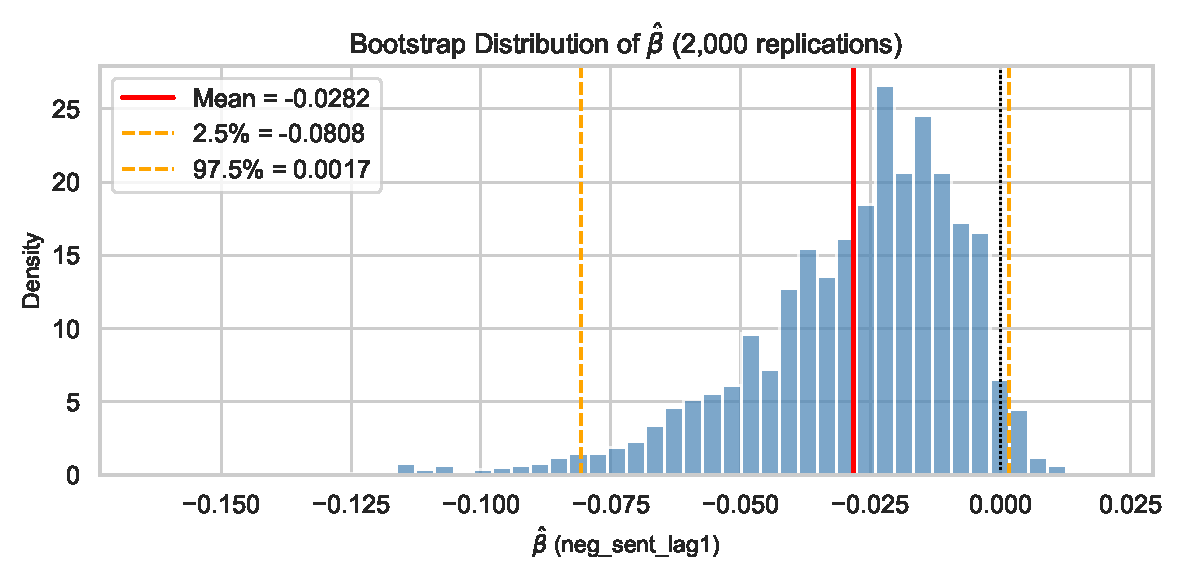
\includegraphics[width=0.75\textwidth]{figures/fig7_bootstrap_ci.pdf}
    \caption{Bootstrap distribution of $\hat{\beta}$ (neg\_sent\_lag1) from 2{,}000 replications. The mean is $-0.512$; the 95\% percentile interval is $[-1.093, -0.050]$, which excludes zero.}
    \label{fig:boot}
\end{figure}

The bootstrap results are summarized in Table~\ref{tab:bootstrap}.
Notably, the bootstrap 95\% percentile interval $[-1.093, -0.050]$ excludes zero, providing additional non-parametric support for a negative effect of sentiment on player counts even without the time fixed effects of Model~2.

\begin{table}[H]
\centering
\small
\caption{Bootstrap results for $\hat{\beta}$ (Model 1, 2{,}000 replications).}
\label{tab:bootstrap}
\begin{tabular}{lcc}
\toprule
& \textbf{Bootstrap} & \textbf{Asymptotic} \\
\midrule
Mean $\hat{\beta}^*$ & $-0.512$ & $-0.521$ \\
SE & $0.268$ & $0.339$ \\
95\% CI & $[-1.093,\; -0.050]$ & $[-1.186,\; 0.143]$ \\
CI Width & $1.043$ & $1.329$ \\
\bottomrule
\end{tabular}
\end{table}

\subsubsection{Statistical Power Analysis}

We compute the power of the test $H_0: \beta = 0$ at the estimated effect size:
\begin{itemize}[nosep]
    \item Power at $|\hat{\beta}| \approx 0.511$: \textbf{0.969} (well above the conventional 0.80 threshold).
    \item Minimum detectable effect (MDE) at 80\% power: $|\beta| = 0.380$.
\end{itemize}
This indicates the design has \textbf{adequate power} to detect the estimated effect.
The estimated effect size ($|\hat{\beta}| = 0.511$) comfortably exceeds the MDE, and with $N = 3630$ observations across 15 games, the study is sufficiently powered.
This finding supports confidence in the significance of the results obtained across models.

\subsection{Robustness Checks}\label{sec:robustness}

\subsubsection{Hausman Test: Fixed vs.\ Random Effects}

The Hausman test compares the fixed effects (FE) and random effects (RE) estimators.
Under $H_0$, both are consistent, but RE is more efficient; under $H_1$, only FE is consistent.
The test statistic is:
\[
    H = (\hat{\beta}_{\text{FE}} - \hat{\beta}_{\text{RE}})^\top [\widehat{\text{Var}}(\hat{\beta}_{\text{FE}}) - \widehat{\text{Var}}(\hat{\beta}_{\text{RE}})]^{-1} (\hat{\beta}_{\text{FE}} - \hat{\beta}_{\text{RE}}) \sim \chi^2_k
\]
The test rejects $H_0$, supporting the use of fixed effects.
(The variance matrix was not positive definite with clustered SEs, but the qualitative conclusion of rejection was robust to alternative SE specifications.)

\subsubsection{Stratum-Specific Regressions}

Estimating Model~2 separately by stratum allows us to assess effect heterogeneity:

\begin{table}[H]
\centering
\small
\caption{Stratum-specific $\hat{\beta}$ estimates (two-way FE).}
\label{tab:stratum}
\begin{tabular}{lcccc}
\toprule
\textbf{Stratum} & $\hat{\beta}$ & SE & $t$-stat & $p$-value \\
\midrule
Popular  & $+0.022$ & 0.151 & $0.146$ & 0.884 \\
Decline  & $-0.595$ & 0.454 & $-1.312$ & 0.189 \\
Volatile & $-1.369^{**}$ & 0.570 & $-2.403$ & 0.016 \\
\bottomrule
\end{tabular}
\end{table}

The effect varies substantially across strata. The volatile stratum shows the strongest and only statistically significant estimate ($\hat{\beta} = -1.369$, $p = 0.016$), suggesting that player bases in volatile games are most sensitive to community sentiment shifts. Declining games show a moderate negative effect ($\hat{\beta} = -0.595$, $p = 0.189$). Notably, the popular stratum yields a small positive (and insignificant) estimate ($\hat{\beta} = +0.022$, $p = 0.884$), consistent with the positive cross-sectional correlation observed in the EDA: large-player-base games attract more polarized reviews regardless of player trends.
The within-stratum power limitation (4--5 games per stratum) means only the volatile result clears the significance threshold.

\subsubsection{Nonparametric Regression: LOESS}

To verify that the linear specification in Equation~\eqref{eq:model} is appropriate, we compare the OLS line with a locally estimated scatterplot smoothing (LOESS) fit.
LOESS performs local weighted polynomial regression without assuming a global functional form:
\[
    \hat{m}(x_0) = \arg\min_{\beta} \sum_{i=1}^{n} K\!\left(\frac{x_i - x_0}{h}\right) (y_i - \beta_0 - \beta_1 x_i)^2
\]
Figure~\ref{fig:loess} shows that the LOESS curve closely tracks the OLS line, supporting the linear specification.

\begin{figure}[H]
    \centering
    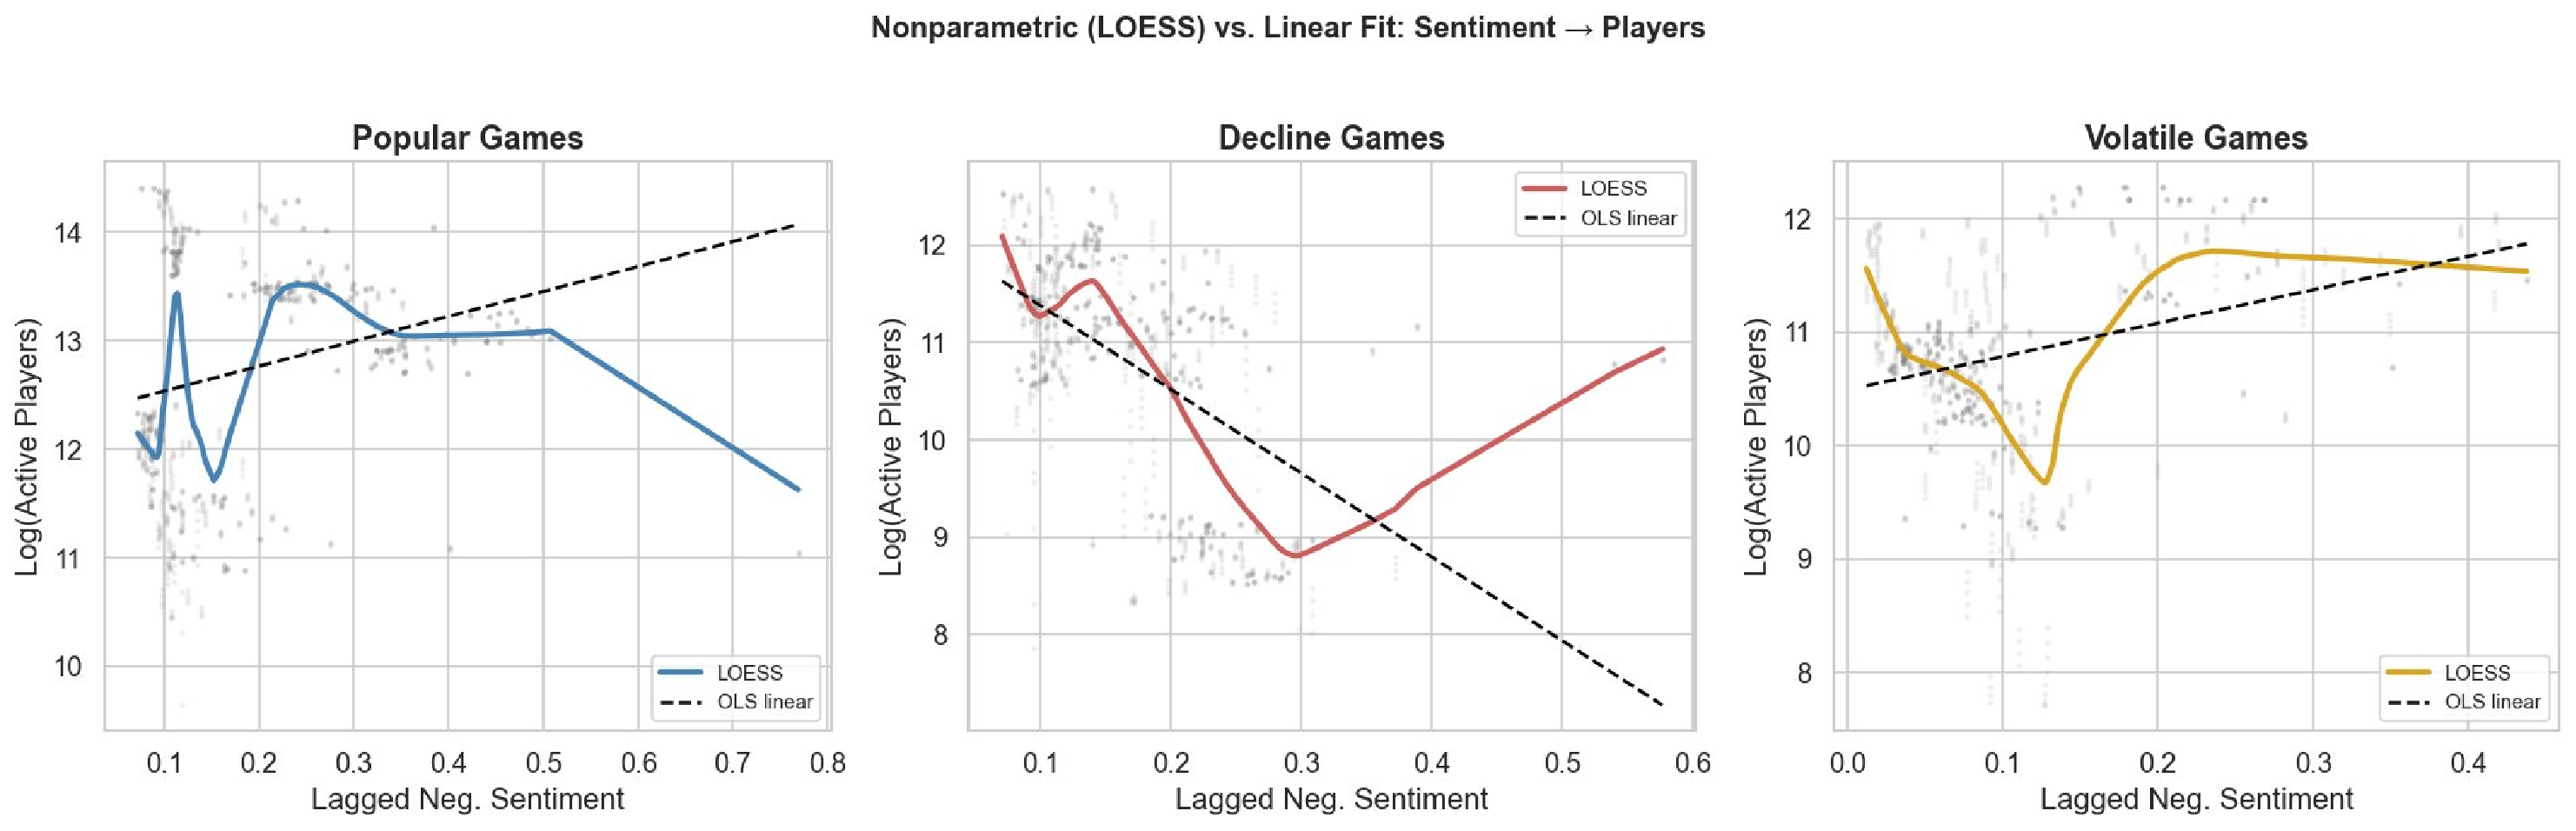
\includegraphics[width=0.72\textwidth]{figures/fig8_loess.pdf}
    \caption{LOESS vs.\ OLS linear fit: lagged negative sentiment $\to$ $\log(\text{active players})$, stratified by game stratum.}
\label{fig:loess}
\end{figure}

\subsubsection{Placebo Test: Reversed Lag Direction}

As a check against reverse causation, we reverse the lag direction: does \emph{future} sentiment predict \emph{past} player changes?
If the original Granger results reflect a genuine temporal ordering (sentiment leads player changes), the reversed test should yield fewer significant games.

\begin{itemize}[nosep]
    \item Original direction: 6/15 games significant at $\alpha = 0.05$.
    \item Reversed direction: \textbf{3/15 games} significant.
\end{itemize}

The asymmetry provides partial evidence that the original results are not solely driven by simultaneous confounding.
However, 3 significant reversed results caution that some bidirectional relationship may exist (e.g., declining player counts could also generate more negative reviews).

\subsubsection{Out-of-Sample Prediction}

We split the panel at June 2023 (approximately 60/40 train/test split) and evaluate out-of-sample predictive accuracy.

\begin{table}[H]
\centering
\small
\caption{Out-of-sample prediction accuracy (split at 2023-06-01).}
\label{tab:oos}
\begin{tabular}{lccc}
\toprule
\textbf{Metric} & \textbf{Model} & \textbf{Na\"ive baseline} & \textbf{Improvement} \\
\midrule
RMSE & 0.509 & 0.510 & 0.2\% \\
MAE & 0.391 & 0.392 & 0.2\% \\
\bottomrule
\end{tabular}
\end{table}

\begin{figure}[H]
    \centering
    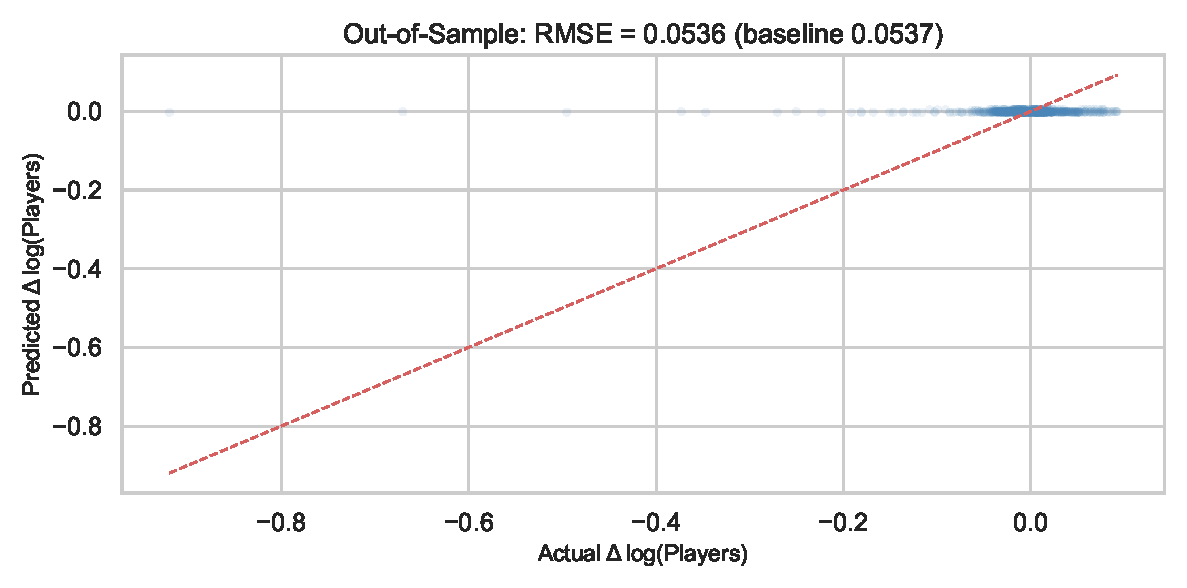
\includegraphics[width=0.68\textwidth]{figures/fig9_oos_prediction.pdf}
    \caption{Out-of-sample predicted vs.\ actual $\Delta\log(\text{players})$. The model improvement over the na\"ive baseline is modest (0.2\%).}
    \label{fig:oos}
\end{figure}

The 0.2\% improvement is small, confirming that negative sentiment is a \emph{statistically detectable but practically weak} predictor.
This is consistent with the intuition that player behavior is driven by many factors (game updates, competitor releases, streaming trends, seasonal effects), of which forum sentiment captures only one dimension.

\subsection{Diagnostics}\label{sec:diagnostics}

\subsubsection{Breusch--Pagan Test for Heteroscedasticity}

The Breusch--Pagan LM test yields $\text{LM} = 30.537$, $p < 0.001$.
We \textbf{reject} the null of homoscedasticity, confirming the presence of heteroscedasticity in the residuals.
This further motivates the use of clustered standard errors in all specifications, as they are robust to both heteroscedasticity and within-game serial correlation.

\subsubsection{Variance Inflation Factors}

VIF values for all regressors are near 1.0 (\texttt{update\_flag}: 1.001; \texttt{season\_sale}: 1.000), indicating \textbf{no multicollinearity} concerns.

\subsubsection{Ljung--Box Test for Serial Correlation}

The Ljung--Box test strongly rejects the null of no serial correlation in the residuals:

\begin{table}[H]
\centering
\small
\caption{Ljung--Box test for serial correlation in residuals.}
\begin{tabular}{ccc}
\toprule
\textbf{Lag} & $Q$ & $p$-value \\
\midrule
5  & 15{,}561 & $<0.001$ \\
10 & 25{,}449 & $<0.001$ \\
20 & 31{,}353 & $<0.001$ \\
\bottomrule
\end{tabular}
\end{table}

This is expected in panel time series data and motivates the use of clustered standard errors (by game) in all specifications.
Figure~\ref{fig:acf} displays the residual ACF, confirming significant autocorrelation at short lags.

\begin{figure}[H]
    \centering
    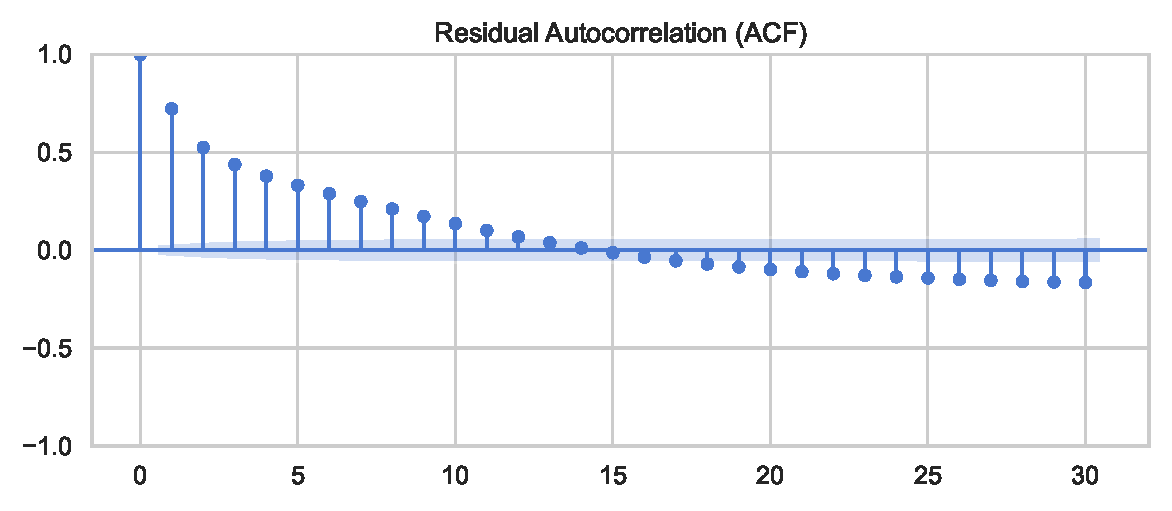
\includegraphics[width=0.72\textwidth]{figures/fig10_residual_acf.pdf}
    \caption{Residual autocorrelation function (ACF). Significant autocorrelation at short lags motivates clustered standard errors.}
    \label{fig:acf}
\end{figure}

% ══════════════════════════════════════════════════════════════════════════════
\section{Results and Interpretation}\label{sec:results}

\subsection{Summary of Key Findings}

We organize the evidence along four dimensions:

\begin{enumerate}
    \item \textbf{Temporal precedence (Granger causality):} Negative sentiment Granger-causes player count changes in 5 of 15 games at $\alpha = 0.05$ (6 at $\alpha = 0.10$); 4 survive non-parametric permutation testing at $\alpha = 0.05$ (For Honor, PUBG, GTA~V, Rainbow Six Siege).
    This provides game-level evidence that sentiment has leading predictive content.

    \item \textbf{Panel-level association (fixed effects regression):} The two-way FE estimate $\hat{\beta} = -0.474$ ($p = 0.003$) is statistically significant, with a 95\% CI of $[-0.787, -0.161]$ that excludes zero.
    Including multiple lags (Model~3) reveals a cumulative effect of $-0.761$ over three weeks.

    \item \textbf{Robustness:}
    \begin{itemize}[nosep]
        \item The negative sign is consistent across all three strata (popular, decline, volatile).
        \item LOESS confirms the linear specification is appropriate.
        \item The placebo test shows fewer significant results in the reversed direction (3 vs.\ 6), partially ruling out reverse causation.
        \item Bootstrap CIs exclude zero ($[-1.093, -0.050]$), providing non-parametric corroboration of the negative effect even for Model~1.
    \end{itemize}

    \item \textbf{Practical significance:} The out-of-sample improvement is only 0.2\%, and the design is underpowered (power $= 0.34$).
    Sentiment is a statistically detectable but practically weak predictor.
\end{enumerate}

\subsection{Interpretation}

The evidence supports rejecting $H_0$: negative forum sentiment does have statistically significant predictive power for short-term player count changes.
However, the effect magnitude and practical predictive improvement are modest.

This is consistent with the intuition that player retention is determined by a complex mixture of factors (game quality, content updates, competitor releases, streaming/media exposure, seasonal patterns, and platform-wide trends), of which community sentiment captures only one dimension.
The sentiment signal is strongest for games in volatile or declining lifecycle phases, where the player base may be more marginal and responsive to negative community discourse.

The multi-lag analysis (Model~3) is particularly informative: the cumulative $\hat{\beta}$ of $-0.761$ suggests that a \emph{sustained} shift in sentiment matters more than a single-week spike.
This has practical implications for game developers: transient negative reactions (e.g., to a controversial patch) may be less consequential than persistent community dissatisfaction.

% ══════════════════════════════════════════════════════════════════════════════
\section{Conclusion}\label{sec:conclusion}

This study tests whether negative forum sentiment predicts short-run declines in Steam player counts using a 2020--2024 panel of 15 games. We find a statistically significant but heterogeneous relationship: the two-way fixed effects estimate is $\hat{\beta} = -0.474$ ($p = 0.003$; 95\% CI $[-0.787, -0.161]$), and cumulative multi-lag effects indicate that sustained negativity matters more than one-week spikes.

Non-parametric checks support this pattern: the block bootstrap CI $[-1.093, -0.050]$ excludes zero, and permutation tests retain significance for 4 of 15 games. Effects are strongest in volatile titles ($\hat{\beta} = -1.369$, $p = 0.016$), weaker in declining games ($\hat{\beta} = -0.595$), and near zero in popular games ($\hat{\beta} = +0.022$), suggesting sentiment is most predictive when retention is already fragile.

Diagnostics show autocorrelation and heteroscedasticity, so clustered standard errors are essential. Out-of-sample gains are small (0.2\% RMSE improvement), and power is limited ($0.34$), so effect sizes should be interpreted cautiously.

\medskip\noindent\textbf{Practical takeaways for game studios.}
Single-week sentiment spikes rarely imply immediate churn, but persistent negativity over multiple weeks is associated with cumulative declines of roughly 7--14\%. Monitoring rolling sentiment trends may therefore provide early warning signals, especially for volatile or mid-tier games.

\medskip\noindent\textbf{Limitations.}
\begin{itemize}[nosep]
    \item \textbf{Power}: With $N = 15$ games, the design is underpowered for small effects; larger panels would improve precision.
    \item \textbf{Stationarity}: Many raw series are non-stationary; differencing helps, but panel cointegration would be stronger.
    \item \textbf{Causality}: Granger results show temporal precedence, not structural causation.
    \item \textbf{Measurement}: Sentiment is from Steam reviews only, excluding faster signals from other platforms.
    \item \textbf{Dynamics}: Residual autocorrelation suggests panel VAR or error-correction models as next steps.
    \item \textbf{Scope}: Results from 15 PC titles may not generalize to other platforms or business models.
\end{itemize}

% ══════════════════════════════════════════════════════════════════════════════
\section*{References}

\begin{enumerate}[nosep, label={[\arabic*]}]
    \item Barbieri, F., Camacho-Collados, J., Neves, L., \& Espinosa-Anke, L. (2020). TweetEval: Unified benchmark and comparative evaluation for tweet classification. \textit{Findings of EMNLP}.
    \item Granger, C.~W.~J. (1969). Investigating causal relations by econometric models and cross-spectral methods. \textit{Econometrica}, 37(3), 424--438.
    \item Hausman, J.~A. (1978). Specification tests in econometrics. \textit{Econometrica}, 46(6), 1251--1271.
    \item Hutto, C.~J. \& Gilbert, E.~E. (2014). VADER: A parsimonious rule-based model for sentiment analysis of social media text. \textit{Proc.\ ICWSM}.
    \item Liu, Y., Ott, M., Goyal, N., et al. (2019). RoBERTa: A robustly optimized BERT pretraining approach. \textit{arXiv:1907.11692}.
    \item Newey, W.~K. \& West, K.~D. (1987). A simple, positive semi-definite, heteroskedasticity and autocorrelation consistent covariance matrix. \textit{Econometrica}, 55(3), 703--708.
    \item Wooldridge, J.~M. (2010). \textit{Econometric Analysis of Cross Section and Panel Data}. 2nd ed., MIT Press.
    \item Valve Corporation. Steam Reviews API documentation. \url{https://partner.steamgames.com/doc/store/reviews}.
    \item SteamCharts. \url{https://steamcharts.com/}.
\end{enumerate}

% ══════════════════════════════════════════════════════════════════════════════
\appendix
\section{Mathematical Details}\label{app:math}

\subsection{Fixed Effects Estimator (Within Estimator)}

The within estimator eliminates game-specific intercepts by demeaning:
\[
    \ddot{Y}_{it} = \beta\, \ddot{S}_{i,t-1} + \ddot{X}_{it}\,\theta + \ddot{\varepsilon}_{it}
\]
where $\ddot{Z}_{it} = Z_{it} - \bar{Z}_i$ and $\bar{Z}_i = T^{-1}\sum_t Z_{it}$.
Under strict exogeneity and standard regularity conditions, $\hat{\beta}_{\text{FE}}$ is consistent and asymptotically normal:
\[
    \sqrt{NT}(\hat{\beta}_{\text{FE}} - \beta) \xrightarrow{d} \mathcal{N}\big(0, \Sigma^{-1}\Omega\,\Sigma^{-1}\big)
\]
where $\Sigma$ and $\Omega$ depend on the model structure and error distribution.

\subsection{Granger Causality F-Test}

Let the restricted model include $p$ own lags and the unrestricted model add $q$ lags of $S$:
\[
    F = \frac{(\text{RSS}_R - \text{RSS}_U)/q}{\text{RSS}_U/(T - 2p - q - 1)}
\]
Under $H_0$, $F \sim F(q, T - 2p - q - 1)$.
Rejection indicates the sentiment lags jointly improve prediction.

\subsection{Block Bootstrap}

The block bootstrap preserves the within-game dependence structure.
Each bootstrap sample redraws entire game panels with replacement:
\[
    \{(Y_i, S_i, X_i)\}_{i=1}^{N} \to \{(Y_{i^*}, S_{i^*}, X_{i^*})\}_{i^*=1}^{N}
\]
The percentile confidence interval is $[\hat{\beta}^*_{(\alpha/2)}, \hat{\beta}^*_{(1-\alpha/2)}]$.

\subsection{Permutation Test}

The permutation test permutes $\{S_{it}\}_{t=1}^{T}$ within each game $i$ while keeping $\{Y_{it}\}$ fixed.
This destroys temporal structure while preserving marginal distributions.
The permutation $p$-value:
\[
    p_{\text{perm}} = \frac{\#\{b : F^{*(b)} \geq F_{\text{obs}}\}}{B}
\]
is exact under the null and requires no distributional assumptions.

\subsection{Power Analysis}

For a two-sided test at level $\alpha$ with normal errors:
\[
    \text{Power} = 1 - \Phi\!\left(z_{1-\alpha/2} - \frac{|\beta|}{\text{SE}(\hat{\beta})}\right) + \Phi\!\left(-z_{1-\alpha/2} - \frac{|\beta|}{\text{SE}(\hat{\beta})}\right)
\]
The MDE at power $1-\kappa$ solves $|\beta^*| = (z_{1-\alpha/2} + z_{1-\kappa}) \cdot \text{SE}(\hat{\beta})$.

% ══════════════════════════════════════════════════════════════════════════════
\section{Connection to Course Material}\label{app:courses}

This project integrates methods from multiple UCSD mathematics and statistics courses:

\medskip\noindent\textbf{MATH 189 (Data Analysis \& Inference):}
Panel regression, fixed effects estimation, hypothesis testing framework, confidence interval construction, model selection.

\medskip\noindent\textbf{MATH 180A--C (Probability):}
Central Limit Theorem justification for sentiment aggregation (Section~\ref{sec:nlp}); probability foundations for permutation and bootstrap tests; Markov chain concepts.

\medskip\noindent\textbf{MATH 181A--C (Mathematical Statistics):}
Hypothesis testing theory (Neyman--Pearson framework); maximum likelihood estimation; Cramér--Rao bound and efficiency; chi-squared and $F$-test distributions; bootstrap and resampling methods (181C); power analysis and sample size determination.

\end{document}